\documentclass[a4paper,12pt,twocolumn]{article}
\usepackage{tabularx} % extra features for tabular environment
\usepackage{amsmath}  % improve math presentation
\usepackage{graphicx} % takes care of graphic including machinery
\usepackage[margin=1in,letterpaper]{geometry} % decreases margins
\usepackage{cite} % takes care of citations
\usepackage[final]{hyperref} % adds hyper links inside the generated pdf file
\usepackage{booktabs,caption, subcaption, multicol}
\usepackage{threeparttable}
\usepackage{graphicx} 
\usepackage{float}
\hypersetup{
	colorlinks=true,       % false: boxed links; true: colored links
	linkcolor=black,        % color of internal links
	citecolor=black,        % color of links to bibliography
	filecolor=magenta,     % color of file links
	urlcolor=black         
}

\begin{document}

\begin{titlepage}
	\begin{center}
		
		\thispagestyle{empty}
		
		\Huge{
			\textbf{UCD School Of Physics}
		}
		
		\vspace{1cm}	
		
		
\includegraphics[scale=0.08]{UCDLogo.png}
		
		\vspace{1cm}
		
		\large{
			\textbf{PHYC30170 Physics with Astronomy and Space Science Lab 1; \\
				Frequency Dependence of the Skin Depth in a Metal Cylinder \\
				\vspace{1cm}
				22/09/2022 \\
				\vspace{1cm}
				Daragh Hollman}
		} \\
		
	\end{center}
\end{titlepage}

\twocolumn[
\begin{@twocolumnfalse}
	\begin{abstract}
		The aim of this experiment was to investigate the frequency dependence of the skin effect in varying metal cylindrical conductors, and measure their conductivity. This was accomplished by measuring the induced voltage in a pick-up coil wrapped on each cylinder.
	\end{abstract}
\end{@twocolumnfalse}
]

\section{Introduction}
	In this experiment
	
\section{Theory}

	As alternating current flows through a conductor the interaction between the electric and magnetic fields in the conductor distribute the charge carriers, and hence the current, toward the surface of the wire [HYPERPHYSICS]. This process acts in the same way regardless of whether ac current is flowing in the conductor, or if the electric and magnetic fields are induced by another source such as a solenoid [JACKSON].\\
	
	A secondary pick-up coil can be wound around the conductor and due to the increase in electric field because of the charged particles at the surface, a voltage can be measured (as shown in figure \ref{fig:circuit}). Faraday's law of induction presents the voltage across the pick-up coil as a function of time [JACKSON]:
	\begin{equation}
		\scriptsize
		V(t) = - i \omega N_2 \left( \int_{0}^{R} B(r) \cdot 2\pi r dr + \int_{R}^{R'} B_0 \cdot 2\pi r dr \right) e^{i\omega t}
		\label{eq:faraday}
	\end{equation}
	where the first integral represents flux within the sample and the second integral represents flux outside the sample. $N_2$ is the number of turns in the pick-up coil, $R$ the radius of the sample cylinder and $R'$ the mean radius of the pick-up coil.\\
	
	Following the derivations carried out in [MANUAL] it can be shown that Faraday's Law reduces to the following equation for the pick-up voltage as a linear equation dependent on skin depth:
	
	\begin{equation}
		\frac{V}{\nu} = \frac{a}{2} + b\delta
		\label{eq:line}
	\end{equation}\\
	where $a = 2\pi^2 N_2 B_0 (R'^2-R^2)$, $b = 2\pi^2 N_2 B_0 R$ and skin depth, $\delta = (\pi \sigma \mu)^{-1/2}$. This equation can then be used to calculate parameters such as the conductivity and skin depth by plotting $V\nu^{-1}$ against $\nu^{-1/2}$.\\
	
	Therefore, in this experiment to determine the frequency dependence of skin depth we will measure and compare the pick-up voltage with respect to varying frequencies and by equating this to equation \ref{eq:line} the conductivity and skin depth will be calculated.
	
\section{Methodology}
	
	\begin{figure}
		\centering
		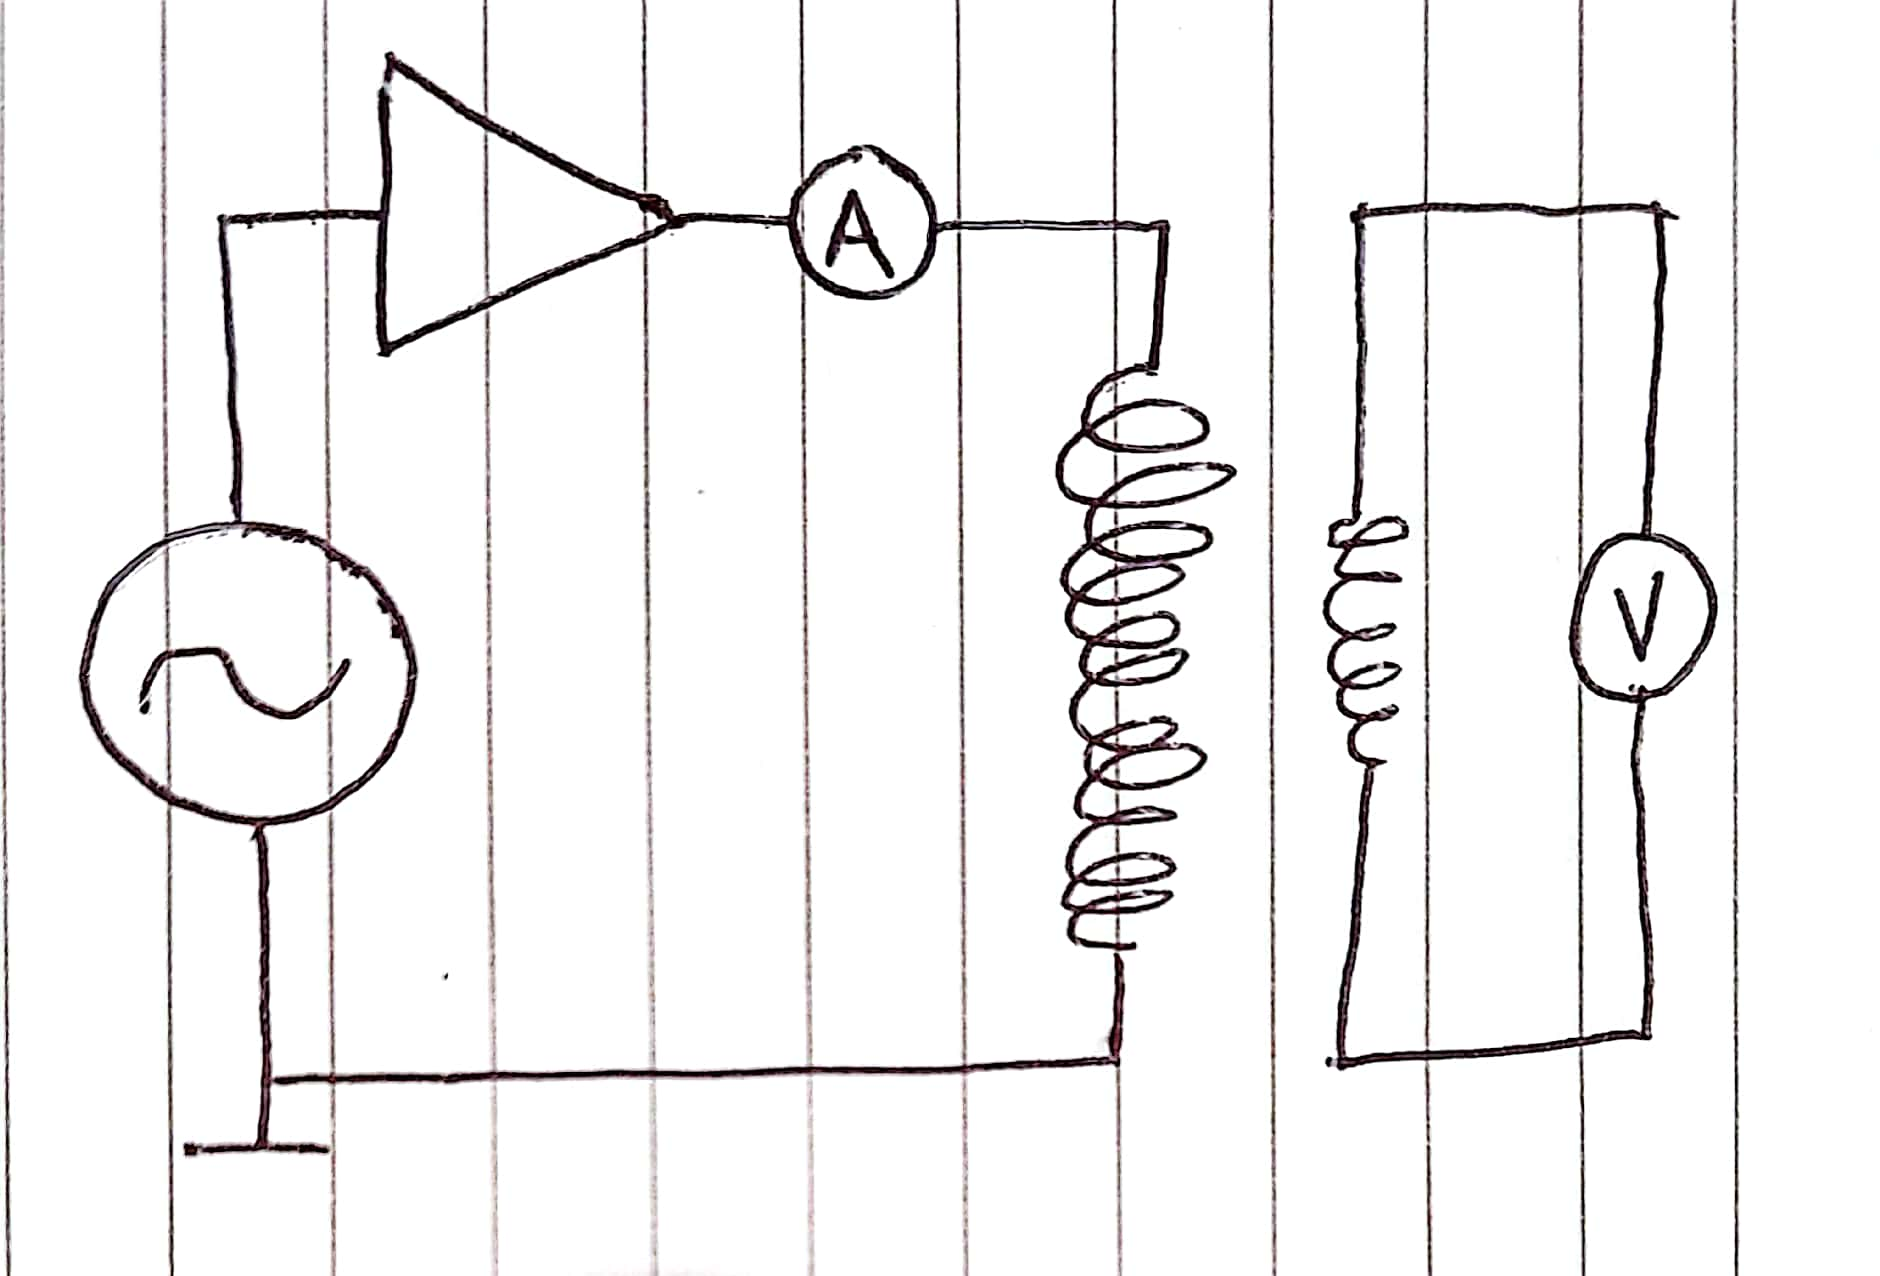
\includegraphics[scale=0.1]{SDcircuit.jpg}
		\captionsetup{font=scriptsize}
		\caption{Circuit diagram of the skin depth apparatus, a AC signal generator is amplified and passed through a solenoid. A signal is induced in the smaller pick-up coil (right) across which the potential is measured.}
		\label{fig:circuit}
	\end{figure}

	\begin{figure}
		\centering
		\includegraphics[scale=0.045]{SDPhoto.jpg}
		\captionsetup{font=scriptsize}
		\caption{Photo of the skin depth apparatus, the metal cylinders were held inside the solenoid (foreground). A duplicate signal from the amplifier was passed to an oscilloscope to check the shape of the waveform was nominal, however no readings were taken from it.}
		\label{fig:photo}
	\end{figure}

	The apparatus was setup as shown in figures \ref{fig:circuit} and \ref{fig:photo}. The induction field was created by a solenoid of length $L_1 = (389 \pm 0.5) \,\text{mm}$ which contained $N_1 = (856 \pm 78)$ turns of an insulated copper wire wound on a hollow tube - which the metal cylinders were inserted into. The signal to this solenoid was created by an AC signal generator and amplified. The rms current was kept constant at $I = (19 \pm 0.1)\,\text{mA}$; Which was adjusted to adjust for each frequency due to the change in reactance. Although the accuracy of the ammeter used was higher, a larger uncertainty was used in practice to account for the very high sensitivity of adjusting the amplitude of the signal generator's output.\\
	
	Four cylinders were used, all of the same dimensions ($L = (389 \pm 0.5)\,\text{mm}$ $R = (4.8 \pm 0.25)\,\text{mm}$): Copper, aluminum, brass and steel. Each cylinder was wrapped at its midpoint with a pick-up coil, of a thicker insulated copper wire than the solenoid, containing $(100 \pm 10)$ turns. The tail ends of this coil were routed down the length and outside of the solenoid to where they could be connected to a voltmeter to take measurements.\\
	
	Voltages were measured from this pick-up coil for 30 frequencies between $6.5 \,\text{kHz}$ and $62.5 \,\text{kHz}$. This range was decided upon based on the results of the same skin depth experiment carried out by H.D. Wiederick and N. Gauthier [MANUAL]. These data were recorded and the voltage divided by the frequency ($V \nu^{-1}$) was plotted against the inverse of the square root of the frequency ($\nu ^{-1/2}$). This was repeated for all four cylinders.
	
\section{Results and Analysis}
	
	The voltage divided by the frequency ($V \nu^{-1}$) was plotted against the inverse of the square root of the frequency ($\nu ^{-1/2}$) for each cylinder in figures \ref{fig:copperGraph}, \ref{fig:aluminiumGraph}, \ref{fig:brassGraph} and \ref{fig:steelGraph}. Scatter plots were used to display the data and a linear least squares fit was used to calculate the slope of the linear portion of the data. At higher frequencies the data deviates significantly from the expected linear result and is hence excluded from the fit calculation. This was unexpected although it is likely due to the skin depth at high frequencies becoming comparable to the air gap between the pick-up coil and the conductor. This leads to a breakdown in the assumptions made in the theory[MANUAL].\\
	
	From the calculated slopes, the conductivity of each material was determined by comparing expression \ref{eq:line} with the linear fit to solve for the conductivity as shown in table \ref{tab:conductivity}.\\
	
	\begin{table}[]
		\centering
		\resizebox{0.8\columnwidth}{!}{%
			\begin{tabular}{@{}ll@{}}
				\toprule
				Sample    & Conductivity ($10^6$ S m$^{-1}$) \\ \midrule
				Copper    & 123.9 $\pm$ 54.5      \\
				Aluminium & 60.7  $\pm$ 17.9      \\
				Brass     & 12.5  $\pm$ 3.7       \\
				Steel     & 4.5   $\pm$ 1.4       \\ \bottomrule
			\end{tabular}%
		}
		\captionsetup{font=scriptsize}
		\caption{The calculated conductivity for each metal cylinder. The uncertainties shown were calculated using error propagation. See appendix [PYTHON ERROR]}
		\label{tab:conductivity}
	\end{table}
	
	It could be inferred from the results that the steel was a carbon steel based on the conductivity calculated using its permeability.
	
	Discuss relative mu with respect to ferrous metals.
	
	Extra care was placed into the analysis of the error propagation, particularly pertaining to the voltage.
	
	Due to having higher voltages, the relative error on the brass and particularly the steel graph was reduced.
	
	\begin{figure*}
		\centering
		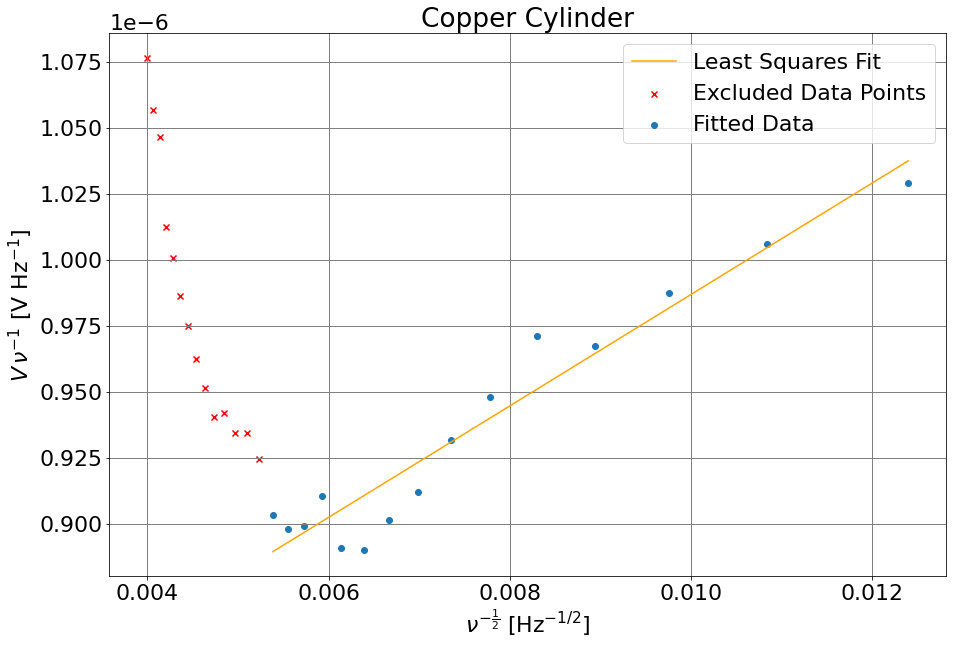
\includegraphics[scale=0.4]{copperGraph.png}
		\captionsetup{font=scriptsize}
		\caption{Plot of the linear relationship between $V\nu^{-1}$ against $\nu^{-1/2}$ for the copper conductor. The copper sample showed the earliest deviation from the expected linear path starting from $28 \,\text{kHz}$. The data points marked in red were excluded from the least squares fit.}
		\label{fig:copperGraph}
	\end{figure*}
	\begin{figure*}
		\centering
		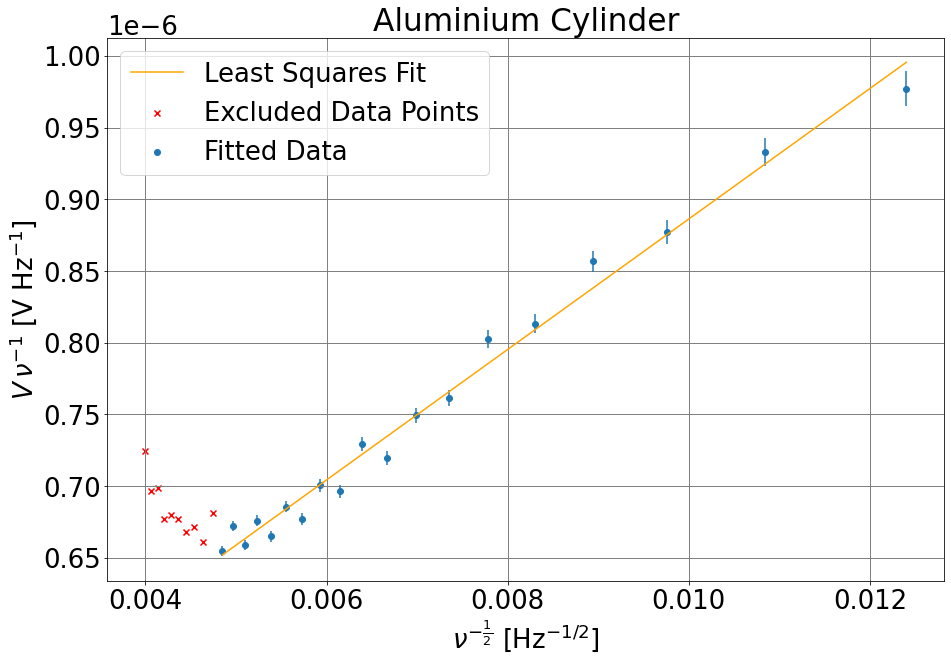
\includegraphics[scale=0.4]{aluminiumGraph.png}
		\captionsetup{font=scriptsize}
		\caption{Plot of the linear relationship between $V\nu^{-1}$ against $\nu^{-1/2}$ for the aluminium conductor. This sample also deviated from the expected linear path however this was not until $42 \,\text{kHz}$. The data points marked in red were excluded from the least squares fit.}
		\label{fig:aluminiumGraph}
	\end{figure*}
	\begin{figure*}
		\centering
		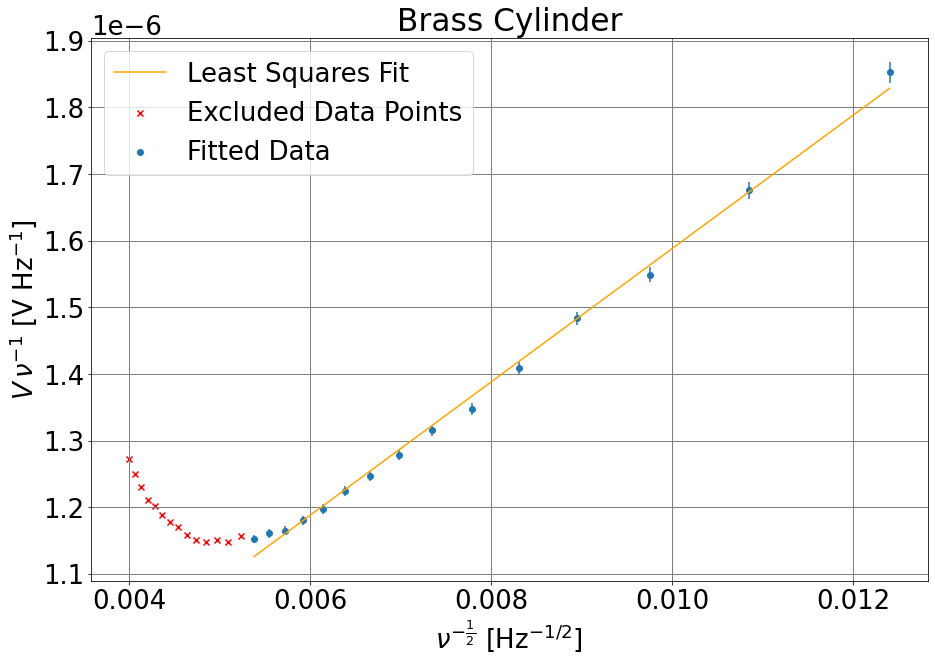
\includegraphics[scale=0.4]{brassGraph.png}
		\captionsetup{font=scriptsize}
		\caption{Plot of the linear relationship between $V\nu^{-1}$ against $\nu^{-1/2}$ for the brass conductor. This sample also deviated from the expected linear path however this was not until $36 \,\text{kHz}$. The data points marked in red were excluded from the least squares fit.}
		\label{fig:brassGraph}
	\end{figure*}
	\begin{figure*}
		\centering
		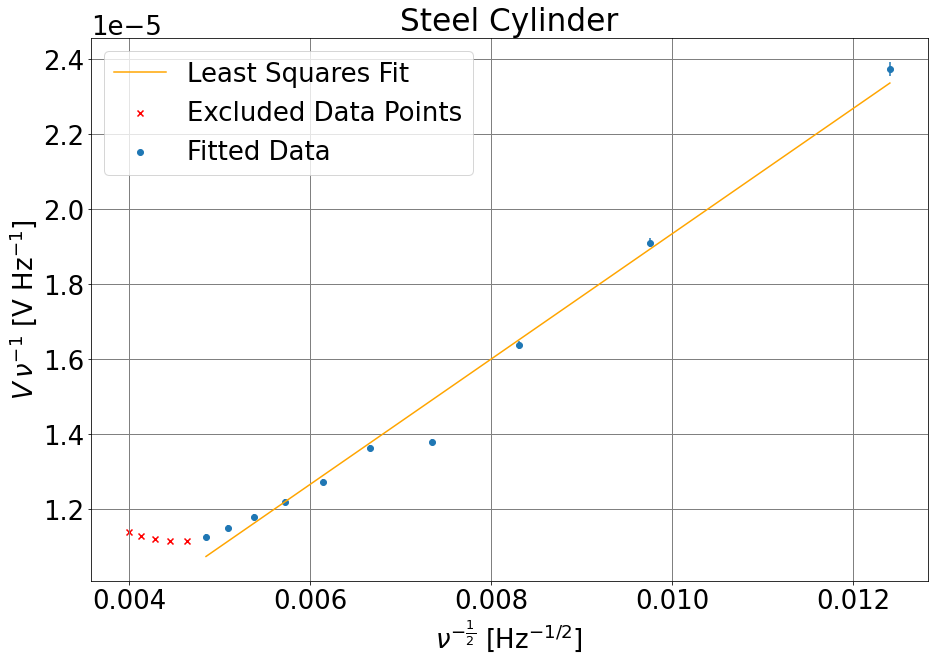
\includegraphics[scale=0.4]{steelGraph.png}
		\captionsetup{font=scriptsize}
		\caption{Plot of the linear relationship between $V\nu^{-1}$ against $\nu^{-1/2}$ for the aluminium conductor. Due to the increased permeability of steel the voltage was approximately one order of magnitude higher. This greatly reduced the calculated error on the data points however some outliers do still remain. The data points marked in red were excluded from the least squares fit.}
		\label{fig:steelGraph}
	\end{figure*}
	

\section{Conclusion}
	

\newpage
\begin{thebibliography}{}
	
	
\end{thebibliography}

	

\newpage

\section*{Appendices}
	
	
\end{document}
